In this chapter we will describe the technical realization of the framework. We can observe in the figure \ref{fig:ClassDiagram} how the most important entities of the framework are related. And each of them are described in the next sections. We will describe as well the implemented database; which it's model is shown on the figure: \ref{fig:DB_001} and the Libraries used in the realization of the framework.

	\begin{figure}\centering
		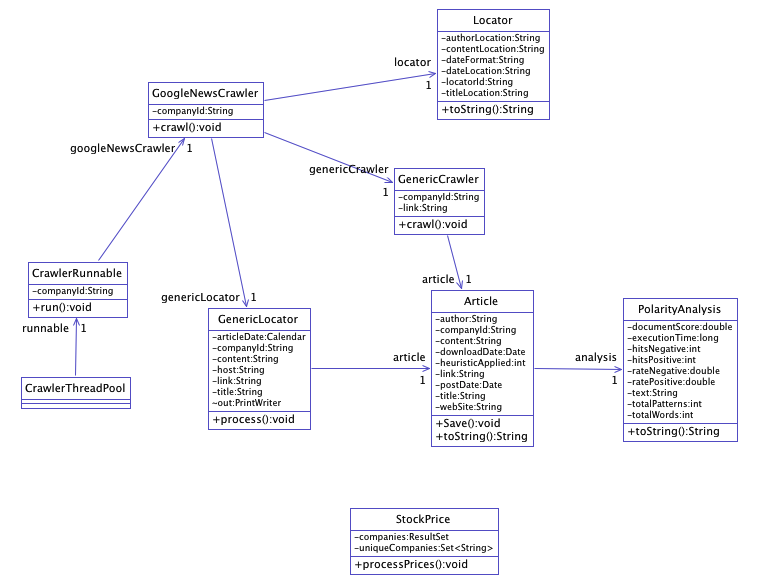
\includegraphics[scale=0.55]{ClassDiagram}
		\caption{Class diagram of the framework.}\label{fig:ClassDiagram}
	\end{figure}

\section{Configuration Files}

Because of the nature of the thesis, it's suitable to manage configuration files in order to change the behavior of the framework without changing a single line of code, and of course not to \emph{hardcode} text or any string inside the code. The framework consists on 10 configuration files that contains around 40 different variables that can be set. We will describe each of them.

\begin{itemize}
	\item \emph{main.properties}: This configuration file was conceived for the user not to input 9 different parameters when he will run the application on the console. It contains only the paths for the other configuration files. We will introduce the required format, it's not necessary that the files have a strict name. What is mandatory is not to change the name of the variables (in the left).
	
\begin{lstlisting}
genericConstantsProperties = /Path/constants.properties
crawlerProperties = /Path/crawler.properties
databaseProperties = /Path/database.properties
dateFormatProperties = /Path/dateFormat.properties
filesProperties = /Path/files.properties
googleNewsProperties = /Path/googleNews.properties
jsoupProperties = /Path/jsoup.properties
locatorsProperties = /Path/locators.properties
priceProperties = /Path/priceEndPoint.properties
\end{lstlisting}
	
	\item \emph{constants.properties}:  This file is simple but important as well. Because here we define the debug mode of the application; and it defines the amount of output in console, if we will use the generic locator and if we will save the article or if it will be in simulation mode.
	
\begin{lstlisting}
DEBUG = true
USE_GENERIC_LOCATOR = true
SAVE_ARTICLE = true
\end{lstlisting}
	
	\item \emph{crawler.properties}\label{crawlerProperties}: This property file is the most important one for the crawler, because here we define for each host where exactly is the title, date, content and author of one particular article. For example; for the host \url{www.financialexpress.com} after following the procedure explained in \ref{locators}

\begin{lstlisting}
GenericCrawler.source.1 = www.fool.com;h1.xlHeader;div.entry-content;span[itemprop=author]; span.dateline;MMMM dd, yyyy
GenericCrawler.source.11 = www.financialexpress.com;h1;font;div.dateline;div.dateline;MMM dd yyyy
GenericCrawler.source.13 = indiatoday.intoday.in;h1;div.strleft;div.strstrap;div.strstrap;MMMM dd, yyyy
\end{lstlisting}	

	\item \emph{database.properties}: In this file, we will define the connection parameters of the database; host, user name, password, database name, port, and connection string (which is a formatted that would looks like:  \url{jdbc:mysql://localhost:port/DiplomaWork?user=myUser&password=myPassword})

\begin{lstlisting}
DB_HOST = localhost
DB_USER_NAME = myUser
DB_PASSWORD = myPassword
DB_NAME = DiplomaWork
DB_PORT = 8889
DB_CONNECTION_STRING = jdbc:mysql://%s:%s/%s?user=%s&password=%s
\end{lstlisting}

	\item \emph{dateFormat.properties}: In this file we define the possible date formats that we can find in the different Web pages. If we find more date formats in any other Web page, we just add a new row in this file with the regular expression of the desired date format.
	
\begin{lstlisting}
date.regex.2 = ([0-9]{4}-[0-9]{1,2}-[0-9]{1,2})
date.regex.5 = ([0-9]{1,2}(-|/)[0-9]{1,2}(-|/)[0-9]{2,4})
\end{lstlisting}

	\item \emph{files.properties}: Here we define a list of several files for several purposes. Here we define where the GATE home folder is, the Pluggin folder, the JAPE grammar file, and the \emph{bag of words} (positive, negative and stop words)

\begin{lstlisting}
GATE_HOME_FOLDER = /Applications/GATE_Developer_7.1
GATE_PLUGIN_FOLDER = /plugins
GATE_JAPE_FILE = /files/patterns.jape
WORD_BANK_NEGATIVE = /files/negative-words.txt
WORD_BANK_POSITIVE = /files/positive-words.txt
WORD_BANK_STOP = /files/stop-words.txt
\end{lstlisting}

	\item \emph{stocks.properties}: This File contains the code of the stocks that will be crawled in the framework. We show here only a small part of the file. 
	
\begin{lstlisting}
company.1 = MMM
company.2 = AXP
company.3 = T
company.4 = BA
company.5 = CAT
company.6 = CVX
company.7 = CSCO
company.8 = KO
company.9 = DD
company.10 = XOM
\end{lstlisting}

	\item \emph{googleNews.properties}: To explain this file we will refer to the Locators (\ref{locators}), where we explain how to get the articles from google news. And here, we define the parameters (If we observe with detail, in the figures: \ref{fig:News_001}, \ref{fig:News_002}, \ref{fig:News_003}, \ref{fig:News_004}  we can see the name/id from the tag that contains every piece of information) how to do it; the url of the news end point, the location in the Web page of the main container, title, link, date. 
	
\begin{lstlisting}
GOOGLE_NEWS_END_POINT = https://www.google.com/finance/company_news?q=%s&start=%s&num=%s
GOOGLE_NEWS_RESULTS_PER_PAGE = 50
GOOGLE_NEWS_CONTAINER = div#news-main
GOOGLE_NEWS_ROW_ID = div.g-section.news.sfe-break-bottom-16
GOOGLE_NEWS_ROW_TITLE_ID = n-cn-
GOOGLE_NEWS_ROW_SOURCE = src
GOOGLE_NEWS_ROW_DATE = date
\end{lstlisting}	
	
	\item \emph{jsoup.properties}: In this work we help ourselves with and HTML parser called \emph{JSOUP}, and we have to set up some parameters in this configuration file, in order not to \emph{hardcode} strings in the source code. We define here, the name of the user agent, the url where we are supposed to be referred, if we should ignore the http errors or not, and the time out in order to not to wait so long if some news article host is offline.
	
\begin{lstlisting}
JSOUP_USER_AGENT = Mozilla/5.0 (Windows U WindowsNT 5.1 en-US rv1.8.1.6) Gecko/20070725 Firefox/2.0.0.6
JSOUP_REFERAL_URL = http://www.margaritka.com
JSOUP_IGNORE_HTTP_ERRORS = true
JSOUP_HTTP_SUCCESS_CODE = 200
JSOUP_TIME_OUT = 30000
\end{lstlisting}
	
	\item \emph{locator.properties}: Here, for this property file we will refer as well to the Locators (\ref{locators}) and to the crawler.properties file (\ref{crawlerProperties}). Because, in this file we define how many lines of comment the \emph{crawler.properties} has, what is the element that divides one particular locator in order to make one tag unique or to search in the HTML document for one specific tag. Here we define as well, what will be the minimum size of the article in order for the Generic Locator (\ref{genericLocator})
	
\begin{lstlisting}
LOCATOR_HEADER_LINES_COUNT = 3
LOCATOR_ELEMENT_DIVIDER = ->
LOCATOR_MIN_ARTICLE_SIZE = 200
\end{lstlisting}
	
	\item \emph{priceEndPoint.properties}: In this file, we defined the URL of the price endpoint that we will describe later in the section: {priceRetrieval}, This is a formatted string in which we will be inputing the code of company, the start and also end date; our start date for all the companies will be on January 1st, 2012. This would be a bit inefficient because we would be downloading prices/data that we won't need, but in this case this details was ignored because of the small size of the file that we are downloading (\approx 30 - 50 KB)

\begin{lstlisting}
PRICE_END_POINT = http://ichart.finance.yahoo.com/table.csv? s=%s&a=%d&b=%d&c=%d&d=%d&e=%d&f=%d&g=d&ignore=.csv
FIRST_DAY = 1
FIRST_MONTH = 1
FIRST_YEAR = 2012
\end{lstlisting}
	
\end{itemize}

\section{Singleton}

In our framework we will use the pattern that in software engineering is called \emph{Singleton} \cite{S2014}, which according to the source is: \emph{a design pattern that restricts the instantiation of a class to one object. This is useful when exactly one object is needed to coordinate actions across the system. The concept is sometimes generalized to systems that operate more efficiently when only one object exists, or that restrict the instantiation to a certain number of objects. The term comes from the mathematical concept of a singleton.}

The reason of the \emph{Singleton} is simple but it has a huge impact in the performance of the application. Because it would be non sense to load all libraries, classes, database drivers, database connection and bag of words for every article that we would be analyzing. The application takes around 10 seconds to start; but we should see this ten seconds as an investment, because as we mention we will spend them only once in the startup of the application. The pseudocode is presented in the Algorithm \ref{singletonAlgorithm}, and the part that takes more time is initializing the GATE text mining framework; this framework is presented in the \emph{Part-of-Speech} (\ref{partOfSpeech}). If we will be loading the class for first time, the \emph{unique\_instance = NULL}, so we will load the necessary information, otherwise we will not do anything because the class, frameworks and libraries will be already loaded in memory. The implementation of the class is in the file: \emph{\ul{Singleton.java}}

\begin{algorithm}
\caption{Singleton algorithm}\label{singletonAlgorithm}
\begin{algorithmic}[1]

\IF{$unique\_instance = NULL$}
		\STATE Load the \emph{bag of words};
		\STATE Load the \emph{database drivers};
		\STATE Initialize \emph{GATE Framework};
\ENDIF
\end{algorithmic}
\end{algorithm}

\section{Generic Objects}

In this section, we will describe the generic object and classes that doesn't have to do directly with the implementation of the \emph{News Crawler} and \emph{Sentiment Analysis}.

\begin{itemize}
	\item \emph{\ul{PriceDetail.java}}: We will be using this class in order to parse every day prices for a particular company.
	\item \emph{\ul{Utilities.java}}: This class as it names suggest, contain only utility functions/methods; all of them are public and static; it means that this class doesn't need to be instantiated in order to access it's methods. Some of the methods that can be found here are: counting lines from a text file, count occurrences of a word in a text, count words in a text, simple debug mehtods, extract date from text, correlation, extract querystring parameters from a URL, download web document, logarithm base \emph{2}, logarithm base \emph{n}, implementation of a \emph{NEAR} method, parse and select HTML, memory information, check if a link exists, among others.
\end{itemize}

\section{News Crawler}

This class is one of the two more important, because here we will be implementing the Crawler that will be downloading and extracting the desired information from web pages. As explained earlier, in the section \ref{webCrawler}, we will be relying on the \emph{google news endpoint}, which previously has been analyzed in order to get to know it's structure. The decision of crawling the \emph{Google News endpoint} is because the information is already segmented by category (Because we will only be needing financial news) and company, as well here we have news articles from different providers, and they don't provide (or is not know) a public API to retrieve this information. Sometimes, only a particular provider provides some sort of \emph{pseudo-API} (RSS feeds, usually).

\begin{itemize}
	\item \emph{\ul{GoogleNewsCrawler.java}}: This class is the starting point of the process, where the input data is the code of the company in the stock market. After the instantiation of the class, we will immediately start crawling the page. After this, we will be generating dynamically a link starting from zero (0) to the article number \emph{N}, with offsets of \emph{GOOGLE\_NEWS\_RESULTS\_PER\_PAGE} (50 by default). After this we will download the Web page, and we will be repeating this process until the \emph{stop condition} is fulfill; which is a big change in the HTML structure of the Web page. The process that we will be repeating besides the link generation, will be the link extraction from the already generated link; which contains the article title, date and link; but this process will be in charge of \emph{\ul{GenericCrawler.java}}.
	\item \emph{\ul{GenericCrawler.java}}: This class is in charge of every of the extracted links, and in order to work it will need two parameters; the companyId and extracted link. After this we will download the webpage and according to the \emph{Locator} or \emph{Generic Locator} we will be extracting the article title, date and link, with a high accuracy.	
	\item \emph{\ul{Locator.java}}: This class is used in the \emph{Generic Crawler} and is used in the \emph{Singleton} class in order to create an array with the information in \emph{crawler.properties}. Basically this class is a container in order to extract from the HTML structure the data of our interest.
	\item \emph{\ul{GenericLocator.java}}: This class maybe has a similar name as the previous one, but even if they aim the same objective, which is to extract data from the news article; this class implement a simple heuristic in order to try to get the data from the news article without the implementation of a \emph{Locator} as mentioned in the section \ref{genericLocator} with it's respective algorithm (algorithm \ref{genericLocatorAlgorithm}).
	\item \emph{\ul{Article.java}}: This class is the integration point between the \emph{News Crawler, Sentiment Analysis} and the  \emph{Database}. Basically after an article is successfully parsed in the \emph{News Crawler}, an \emph{Article} object is created and the \emph{Polarity Analysis} class is instantiated inside this class, and finally, after every process is finished the news article is saved. 
\end{itemize}

\section{Sentiment Analysis}

Here, we will be describing the implementation of the theory described in the section \ref{sentimentAnalysis} and it's respective algorithm ({unsupervisedAlgorithm}).

The implementation is in the file: \emph{\ul{PolarityAnalysis.java}}; and it needs only some text as a parameter; here we will remove the stop words and "weird" characters that we could found in the text and we will count the number of positive and negative words founded in the text according to our \emph{bag of words}, and of course, we will count the total number of words. After this, we will use the API of GATE (section: \ref{gate}) in order to extract automatically the words that fulfill the conditions presented early in the table \ref{tab:twoWordPhrases}; as presented in the example in the section \ref{partOfSpeech}, and for each pair of words that fulfill this conditions we will apply the operator \emph{NEAR} in order to take the ten left and rightmost words from the pattern found that fulfill the conditions of the table \ref{tab:twoWordPhrases}. After this, we will calculate the semantic orientation of each phrase found, we will calculate the average and some other useful statistics like: total number of patterns, rate of positive and negative words, execution time, etc. As output the class will return the \emph{score of the document}.

\section{Price retrieval \& Summarization}\label{priceRetrieval}

\emph{\ul{StockPrice.java}}: This class firstly performs a summarization of the data; in order to generate a table which will contain calculated data and general daily statistics about the companies (price, delta, number and percentage of positive and negative articles, etc.) which a posteriori will be correlated in order to present final results faster.

To retrieve the price we will use \url{finance.yahoo.com}, because it has a \gls{Web API} which will allow us to access the stock price data in an easy way. We will find in the file: "priceEndPoint.properties" the link of the \gls{news endpoint} in which we will define basic parameters like: start date and end date.
\\\\
\url{http://ichart.finance.yahoo.com/table.csv} 
\\\\
It's worth to mention that we will consider the close price of the stock. And to get this price we will download the "csv" file, which contains several fields: Date, Open, High, Low, Close, Volume, Adj Close*. In our case we will only need the "Close" field. Unfortunately; until today, there is no way to make a request asking only for the specific field we need, and make the transmission of the file lighter.

First of all, we will count the articles (positive, negative, total) per day, and for that we will be calling a \emph{Stored Procedure} in the database, which for simplicity every time that it's executed will delete al registries from the table, and it will perform calculations per every day were exists news articles, the output data (Ids of the companies) of the \emph{Stored Procedure} will be used to download the prices. 

After this, for each company returned in the output, we will download the prices file and we will parse the mentioned file. Once the data is parsed, we will be saving in the database the final prices.

\section{Startup}

When we are talking about the startup of the application, basically is the class that contains the \emph{main} method; and in our case there are several files, and most of them have been used in the development phase; to test individual parts of the framework. The one class that must be invoked in order to collect the data is \emph{CrawlerThreadPool.java}.

\begin{itemize}
	\item \emph{\ul{CrawlerThreadPool.java}}: As we mention before this is the class that startup the framework. But it has a particularity, instead of the sequential implementation of the framework, this class implements multi-threading in the application, which \emph{speedup} the application considerably; we will verify this fact in the experimental section (\ref{experimentalEvaluation}).
	\item \emph{\ul{CrawlerRunnable.java}}: This is the implementation of a \emph{Runnable} interface for our own purposes, which initialize the \emph{News Crawler} for a particular company.
	\item \emph{\ul{PolarityAnalysisTester.java}}: This class is a tester which help us to estimate the polarity of a particular text.
	\item \emph{\ul{GenericLocatorTester.java}}: For a Web page that has no locator defined, this class implement a tester of the \emph{Generic Locator} to extract the information of our interest.
	\item \emph{\ul{PriceTester.java}}: This class implements a main function for the summarization class \emph{StockPrice.java}.
	\item \emph{\ul{ProcessLinksThreadPool.java}}: This class extracts from the database non-parsed links and try to parse them using the \emph{Generic Locator}.
	\item \emph{\ul{ProcessLinksRunnable.java}}: This is the implementation of a \emph{Runnable} interface for our own purposes, which initialize the \emph{Generic Locator} class.
\end{itemize}


\section{Database}

The database, as we mention earlier in the section \ref{pageRepository}, it will be our \emph{page repository}, and the place where we will keep statistics and the companies that we will be crawling. The entity-relation model was designed in \emph{MySQLWorkbench}; which is an open source visual database design tool. 

The model is quiet simple, it consists on seven tables that we will be discussing here. The entity-relation model is shown on the figure \ref{fig:DB_001}.

	\begin{figure}\centering
		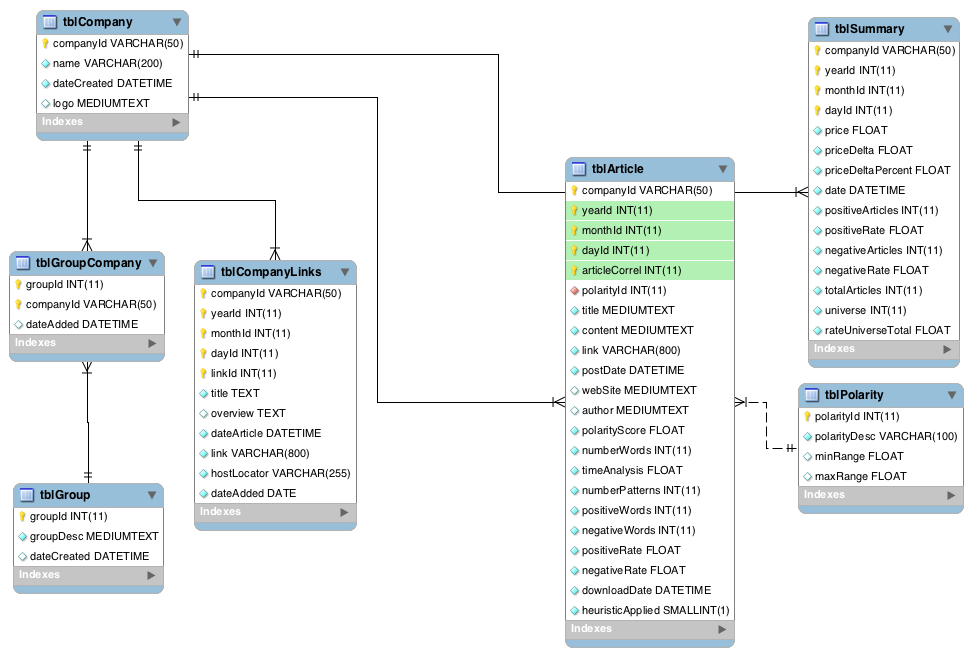
\includegraphics[scale=0.45]{DB_001}
		\caption{Entity-relation diagram of the database.}\label{fig:DB_001}
	\end{figure}

\begin{itemize}
	\item \emph{tblGroup}: We will be storing here the name of one particular group that will contain several companies; this with the objective to consolidate stocks in one particular group, following the idea for example of the industrial average \emph{Dow Jones} which tracks the 30 largest U.S. companies., \emph{NASDAQ} which has several companies that are in \emph{Dow Jones} as well
	\item \emph{tblGroupCompany}: This entity is related directly with \emph{tblGroup} because companies and groups will be joining here. Here we will define which company belongs to which group. This table represents one \emph{many to many} relation. 
	\item \emph{tblCompany}: This entity basically defines a company, with it's code, name and logo.
	\item \emph{tblCompanyLinks}: This entity is a repository of links, if a link goes through the framework, it will be saved here; doesn't matter if it's parsed or not. The parsed links will be in \emph{tblArticle} 
	\item \emph{tblArticle}: Here relies most of the information that we will be using for summarization and experimentation. We identify an article by company, date of publication, and a correlative. And in this entity we will be storing the direction of the polarity, title, content of the article, author, link, score, website, execution time, if heuristic was applied to the link, among others. 
	\item \emph{tblPolarity}: Basically it's a catalog that defines when an article will be positive or negative, with the ranges defined in every tuple.
	\item \emph{tblSummary}: As we know, a company can have several or maybe hundreds of articles per day. And to create a query that would compute this information is would be quiet complex, time consuming and probably messy as well. The objective of this table is to summarize per company and per day the previously collected data: price, delta and delta percent of the stock and number of positive and negative articles collected.
\end{itemize}

Another feature of the database engine used in the framework are the \emph{Stored procedures} and \emph{functions}. And each of the stored procedures used are described here. As a naming convention the \emph{function} names starts with \emph{fn\_} and the  \emph{Stored procedure} names starts with \emph{pr\_}.

\begin{itemize}
	\item \emph{fn\_calculate\_price\_delta}: This function calculates the change (delta) in price of a particular stock from the current day with the previous working day.
	\item \emph{fn\_previous\_working\_day}: This function calculates the previous working day and the result is used by the function \emph{fn\_calculate\_price\_delta} in order to calculate the delta of the price.
	\item \emph{pr\_add\_article}: This stored procedure saves one article to the database, and outputs the correlative of the article generated.
	\item \emph{pr\_init\_database}: This stored procedure initialize the database, we only need to populate the table \emph{tblPolarity}.
	\item \emph{pr\_link\_exist}: Check if a link is already saved in the database; if not it saves it.
	\item \emph{pr\_summarize}: This stored procedure populates the table \emph{tblSummary} daily, with the respective information (Number of positive and negative articles).
	\item \emph{pr\_update\_summary}: This stored procedure is started after the summarization (\emph{pr\_summarize}). After we download the prices, as we mention in the section \ref{priceRetrieval}, and what this procedure does is to update one particular row and calculating the delta of the stock price for that particular day.
\end{itemize}

\section{Librearies}
We will describe briefly the libraries used for the implementation of the framework. 

\begin{itemize}
	\item \emph{GATE}\label{gate}: According to wikipedia \cite{G2014}, \emph{GATE} stands for General Architecture for Text Engineering, which is a Java suite of tools originally developed at the University of Sheffield in beginning of 1995 and now is used worldwide by a wide community of scientists, companies, teachers and students for all sorts of natural language processing tasks, including information extraction in many languages. 
	
	In our work, we have used \emph{GATE} as text pattern extraction; We have mention a practical example in the section {partOfSpeech} using the \emph{GATE} user interface, and in the framework this same example is implemented in code through the \emph{GATE API}.
	
	\item \emph{JSOUP}: is an HTML parser, its “jquery-like” and “regex” selector syntax is very easy to use and flexible enough to get extract any particular information from a Web page. It implements the WHATWG HTML5 specification, and parses HTML to the same DOM as modern browsers do.
	
	In our work, we have used \emph{JSOUP} as HTML parser, in order to download and extract specific data from a Web page that doesn't provide a Web API. Our work is not the kind of work that is written in stone, because we have to be conscious that any change on the structure of the page that we are parsing, we must change the details to specify where the data that we want is located.
	 
\end{itemize}

